% !TEX encoding = UTF-8 Unicode
% !TEX root = SystemTemplate.tex

\documentclass{book}
% !TEX root = SystemTemplate.tex

\usepackage[width=6.5in, height=9.2in, top=1.0in, papersize={8.5in,11in}]{geometry}
\usepackage[pdftex]{graphicx}
%\usepackage{draftwatermark}
\usepackage{amsmath}
\usepackage{amsthm}
\usepackage{amssymb}
%\usepackage{txfonts}
\usepackage{textcomp}
%\usepackage{amsthm}

\usepackage[all]{xy}
\usepackage{fancyhdr}
\pagestyle{fancy}
\usepackage{hyperref}
\usepackage{verbatim}
\usepackage{algorithm}
\usepackage{algorithmic}
\usepackage{array}
\usepackage{color}
\usepackage{listings}
\lstset{language=c,frame=ltrb,framesep=5pt,basicstyle=\normalsize,
 keywordstyle=\ttfamily\color{DarkRed},
identifierstyle=\ttfamily\color{DarkBlue}\bfseries,
commentstyle=\color{OliveGreen},
stringstyle=\ttfamily,
showstringspaces=false,tabsize = 3}
\usepackage{calc}
\usepackage{doxygen}
\usepackage[utf8]{inputenc}
\usepackage{makeidx}
\usepackage{multicol}
\usepackage{multirow}
\usepackage[table]{xcolor}

\definecolor{color02}{rgb}{0.18,0.35,0.59}
\definecolor{color03}{rgb}{0.44,0.59,0.82}
\definecolor{color06}{rgb}{0.35,0.35,0.35}


\newtheorem{summary}{Summary:}
\newtheorem{example}{Example:}


\definecolor{OliveGreen}{cmyk}{0.64,0,0.95,0.40}
\definecolor{DarkBlue}{cmyk}{0.76,0.76,0,0.20}
\definecolor{DarkRed}{cmyk}{0,1,1,0.45}


\def      \RR             {{\mathbb R}} 
\def      \DS            {\displaystyle} 

\setlength{\oddsidemargin}{0mm} 
\setlength{\evensidemargin}{0mm} 

%\SetWatermarkLightness{0.975}
%\SetWatermarkScale{6}
%\SetWatermarkText{\includegraphics{test.png}}

\pagestyle{fancy}
\renewcommand{\chaptermark}[1]{\markboth{#1}{}}
\renewcommand{\sectionmark}[1]{\markright{\thesection\ #1}}
\fancyhf{}
\fancyhead[LE,RO]{\bfseries\thepage}
\fancyhead[LO]{\bfseries\rightmark}
\fancyhead[RE]{\bfseries\leftmark}
\fancyfoot[LE,RO]{Confidential and Proprietary}
%\renewcommand{\headrulewidth}{0.5pt}
%\renewcommand{\footrulewidth}{0pt}
%\addtolength{\headheight}{0.5pt}
%\setlength{\footskip}{0mm}
%\renewcommand{\footruleskip}{0pt}


\definecolor{MSBlue}{rgb}{.204,.353,.541}
\definecolor{MSLightBlue}{rgb}{.31,.506,.741}
\definecolor{MSBlue1}{rgb}{0.18,0.35,0.59}
\definecolor{MSBlue2}{rgb}{0.44,0.59,0.82}
\definecolor{MSBlue3}{rgb}{0.35,0.35,0.35}


\usepackage{titlesec}
\titleformat{\chapter}[display]
{\normalfont\bfseries\color{MSBlue1}}    %\normalfont\bfseries\filcenter}
{\LARGE\thechapter}
{1ex}
{\titlerule[2pt]
\vspace{2ex}%
\LARGE}
[\vspace{1ex}%
{\titlerule[2pt]}]

\definecolor{MSBlue}{rgb}{.204,.353,.541}
\definecolor{MSLightBlue}{rgb}{.31,.506,.741}
\definecolor{MSBlue1}{rgb}{0.18,0.35,0.59}
\definecolor{MSBlue2}{rgb}{0.44,0.59,0.82}
\definecolor{MSBlue3}{rgb}{0.35,0.35,0.35}

%\titleformat*{\section}{\Large\bfseries\sffamily\color{MSBlue}}
%\titleformat*{\subsection}{\large\bfseries\sffamily\color{MSLightBlue}}
%\titleformat*{\section}{\Large\bfseries\color{MSBlue1}}
%\titleformat*{\subsection}{\large\bfseries\color{MSBlue2}}

\titleformat*{\section}{\Large\bfseries\color{MSBlue}}
\titleformat*{\subsection}{\large\bfseries\color{MSLightBlue}}
\titleformat*{\subsubsection}{\large\bfseries\color{MSBlue3}}
\setcounter{secnumdepth}{3}
\renewcommand{\thesubsubsection}{\thesubsection.\alph{subsubsection}}

 % This sets the format.

% Add your title page contents here 
\title{{\color{MSBlue1} \rule{\linewidth}{0.5mm}}\\[2mm] {\huge \bfseries \color{MSBlue1} Product Title }\\[-1mm] {\color{MSBlue1}\rule{\linewidth}{0.5mm}} \\  \vfill
{\LARGE \bfseries \color{MSBlue2} Testing System Project }\\  \vfill 
{\color{MSBlue1} LaTex Samurai} }
\author{\color{MSBlue1}  Julain Brackins \and \color{MSBlue1} Jonathan Dixon \and  \color{MSBlue1} Hafiza Farzami }
\date{\color{MSBlue1} \today}


\begin{document}
\frontmatter
\maketitle


\tableofcontents
\listoffigures
\listoftables
\listofalgorithms


% !TEX root = SystemTemplate.tex

\chapter{Mission}

The mission statement for this project is to create a test suite designed to compile and run C++ projects with various test cases.

\let\cleardoublepage\clearpage  % add mission statement to mission.tex
% !TEX root = SystemTemplate.tex

\chapter{Document Preparation and Updates}

Current Version [1.0.0]
\vspace*{5mm}

{\color{MSBlue3}
\noindent
\textit{Prepared By:}\\
\textit{Hafiza Farzami}\\
%\textit{Team Member \#2}\\
%\textit{Team Member \#3}
}

\vfill
\noindent
{\color{color02} \textit{\textbf{Revision History}}}\\
\begin{tabular}{|>{\raggedright}p{1.5cm}|>{\raggedright}p{3cm}|>{\raggedright}p{1.5cm}|>{\raggedright}p{9cm}|}
\hline
\textit{\textbf{Date}} &  \textit{\textbf{Author}} & \textit{\textbf{Version}} & \textit{\textbf{Comments}}\tabularnewline
\hline
 \textit{\textbf{2/17/14}} & \textit{Hafiza Farzami} & \textit{1.0.0} & \textit{Initial version}\tabularnewline
\hline
%\textit{\textbf{3/4/12}} & \textit{Team Member \#3} & \textit{1.1.0} & \textit{Edited version}\tabularnewline
%\hline
 &  &  & \tabularnewline
 \hline
 &  &  & \tabularnewline
\hline
 &  &  & \tabularnewline
\hline
 &  &  & \tabularnewline
\hline
 &  &  & \tabularnewline
\hline
\end{tabular}
\vfill



 
\mainmatter

%%  Add to the following chapters

% !TEX root = SystemTemplate.tex

\chapter{Overview and concept of operations}

The purpose of this document is to outline the project. That is, it's purpose, the niche it is meant to fill, and it's future.


\section{Scope}
This document covers the details of the project. It describes how it works, what tools it uses, and what has been done so far.


\section{Purpose}
The purpose is to make grading easier for professors and teaching assistants (in particular at the introductory programming level).


\subsection{Major System Component \#1}
Recursive File Searcher

\subsection{Major System Component \#2}
Iterative Executable Tester

\section{Systems Goals}
The primary goal of the project is to aid in the grading of programs. Without a tool to do this, it can be very time-consuming to grade programs that are all meant to be "the same." This is the problem that Assignment Grader is mean to solve.

\section{System Overview and Diagram}
These are the main system components. For clarity, the student's code file has been included in this diagram even though it is an outside resource. See Figure~\ref{systemdiagram} below.

\begin{figure}[tbh]
\begin{center}
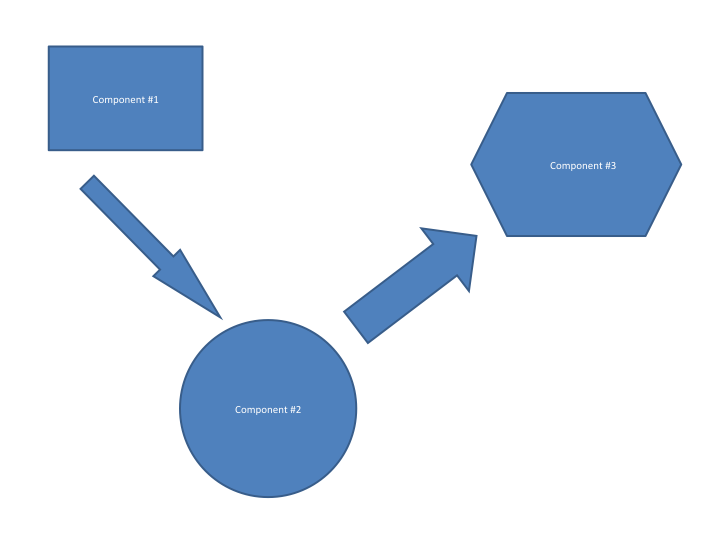
\includegraphics[width=0.75\textwidth]{./diagram}
\end{center}
\caption{System Diagram \label{systemdiagram}}
\end{figure}

\section{Technologies Overview}
Linux (Fedora 19, Ubuntu 13.1) Operating System: Used for basic runtime needs. G+ compiler: used to compile and run both our code and student code. For further information on these two system features, consult Linux documentation.


% !TEX root = SystemTemplate.tex


\chapter{Project Overview}
This section provides some housekeeping type of information with regard to the 
team, project, etc. 



\section{Team Members and Roles}
Describe who was involved and what role(s) were played. 


\section{Project  Management Approach}
This section will provide an explanation of the basic approach to managing the 
project.  Typically, this would detail how the project will be managed through 
a given Agile methodology.  The sprint length (i.e. 2 weeks) and product backlog 
ownership and location (ex. Trello) are examples of what will be discussed.  An 
overview of the system used to track sprint tasks, bug or trouble tickets, and 
user stories would be warranted. 


\section{Phase  Overview}


If the system will be implemented in phases, describe those phases/sub-phases (design, 
implementation, testing, delivery) and the various milestones in this section. 
 This section should also contain a correlation between the phases of development 
and the associated versioning of the system, i.e. major version, minor version, 
revision. 

\section{Terminology and Acronyms}
Provide a list of terms used in the document that warrant definition.  Consider 
industry or domain specific terms and acronyms as well as system specific. 

% !TEX root = SystemTemplate.tex
\chapter{User Stories, Backlog and Requirements}
\section{Overview}

This section covers user stories, backlog and requirements for the system.  

\subsection{Scope}

This document contains stakeholder information, 
initial user stories, requirements, proof of concept results, and various research 
task results. 



\subsection{Purpose of the System}
The purpose of the product is to grade a {\tt <filename>.cpp} file by running test files and comparing the results to answer files, and assigning percentage grade. 


\section{ Stakeholder Information}


This section would provide the basic description of all of the stakeholders for 
the project.

\subsection{Customer or End User (Product Owner)}
Hafiza Farzami is the product owner for this sprint, who is in contact with Dr. Logar regarding requirements, and with the scrum master and technical lead regarding the backlog. 

\subsection{Management or Instructor (Scrum Master)}
Julian Brackins is the scrum master, who breaks the project into smaller tasks, and is in touch with both product owner and technical lead.

%\subsection{Investors}
%Are there any?  Who?  What role will they play? 

\subsection{Developers --Testers}
Jon Dixon is the technical lead for Sprint 2, and is in contact with both Brackins and Farzami regarding the requirements during scrum meetings and through trello notes. Due to the project size and limited number of people, the developers and testers are the same group of people. 

\section{Business Need}
This product is essential for grading computer science programs focused on numerics. The user can save time and not have to do tedious, meticulous work while grading an entire class of students' programs.  

\section{Requirements and Design Constraints}
This section covers the requirements and constraints in order to use this product. 

\subsection{System  Requirements}
This product runs on Linux machines. 

\subsection{Network Requirements}
This software does not require internet connection. 

\subsection{Development Environment Requirements}
There are not any development environment requirements.

\subsection{Project  Management Methodology}
The method used to manage this project is {\tt scrum}. The scrum master met with the product owner, and broke the tasks down to the technical lead. The team meets for ten minutes long scrum meetings to go over the progress, next steps, and impediments. 
 
\begin{itemize}
\item Trello is used to keep track of the backlogs and sprint status
\item Everyone has access to the Sprint and Product Backlogs
\item This project will take three Sprints
\item Each Sprint is two weeks long
\item There are no restrictions on source control 
\end{itemize}

\section{User Stories}
This section contains the user stories regarding functional requirements and how the team broke them down.

\subsection{User Story}
As user I want a testing system, in C++,  so that given a directory of a class containing {\tt <studentsNames>.cpp} files and a test files, it should grade them. 

\subsubsection{User Story Breakdown \#1}
The program needs to be able to "crawl" through directories, be able to identify and run {\tt <studentsNames>.cpp} files using the test files. In other words, the testing suite should be able to process the entire class. 

\begin{figure}[tbh]
\begin{center}
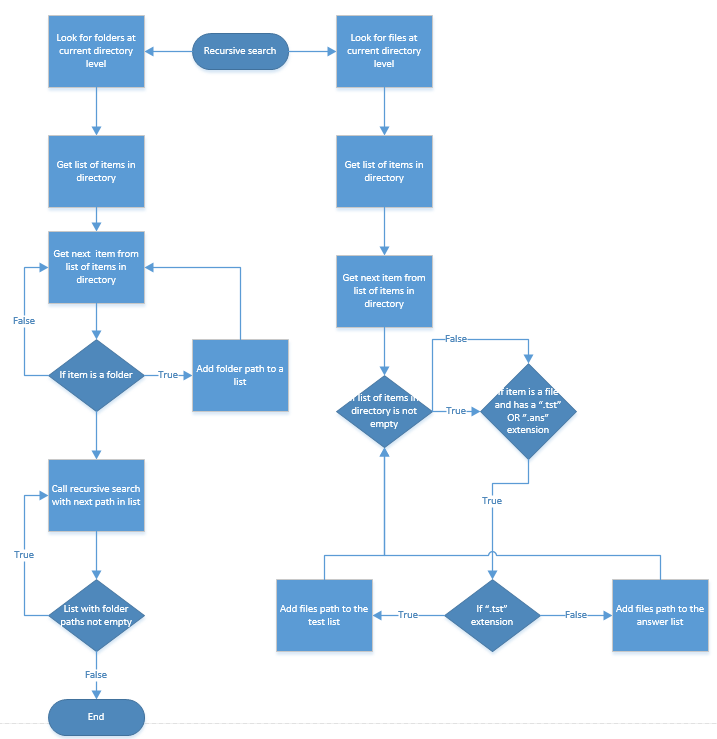
\includegraphics[width=0.75\textwidth]{./Capture}
\end{center}
\caption{Directory Hiararchy Structure \label{directoryhiararchystructure}}
\end{figure}

\subsubsection{User Story Breakdown \#2}
The system needs to grade each individual student, store the result in a log file specific to a given student. The system also has to produce a summary file containing the list of grade percentages of all the students who passed necessary test cases, and the students who failed to pass an important critical case, with the word "FAILED" in the grade column.

\subsubsection{User Story Breakdown \#3}
The individual {\tt <studentName>.log} files will be stored in that student's subdirectory. The summary {\tt .log} file will be located in the root directory.  

The summary file will have the following structure: \\*
\newline
\indent	Student1 Name	\indent Percent grade {\tt or} FAILED \\*
\indent	Student2 Name	\indent Percent grade {\tt or} FAILED \\*
\indent \indent \indent \indent \indent \indent	.				 \\*
\indent \indent \indent \indent \indent \indent	.				 \\*
\indent \indent \indent \indent \indent \indent	.				 \\*
\indent	Studentn Name	\indent Percent grade {\tt or} FAILED
	

\subsubsection{User Story Breakdown \#4}
The system should be able to generate test cases by asking the user about the conditions and constraints.

\let\cleardoublepage\clearpage


% !TEX root = SystemTemplate.tex
\chapter{Design  and Implementation}
 This section describes the design details for the overall system as well as individual major components. As a user, you will have a good understanding of the implemetation details without having to look into the code. Here is the  


\begin{itemize}
  \item Ask if the user if the program needs to generate test cases
  \item If the user's answer is yes: 
	 \begin{itemize}
		\item Get the requirements for test cases
 	 	\item Generate {\tt.tst} files and corresponding {\tt .ans} files using {\tt golden.cpp}
	\end{itemize}
  \item (If no) get all the {\tt .tst} files and add them to a vector 
  \item Get all {\tt .cpp} files and compile them into executable files
  \item Create summary file
  \item For each {\tt .cpp} files in the directory: 
 	\begin{itemize}
 		\item Create {\tt .log} file for current student
		\item For all {\tt .tst} file in the vector:
		\begin{itemize}
			 \item Run student file using current test case
 			\item If pass the increment the number of passed tests, and output the score to student's {\tt .log} file
			 \item If fail, check if it is a critical test, if so, the student has failed, else output the score to the {\tt .log} file
		\end{itemize}
	\end{itemize}
  \item Check if the user wants more cases
  \item If yes, then restart from the beginning
  \item If no:
	\begin{itemize}
  		\item Output student's overall grade to summary file
  		\item Close current student's {\tt .log} file	
	\end{itemize}
  
\item Check if there are more {\tt .cpp} files to be processed
  \item If yes, then repeat the previous steps
  \item If no:
	\begin{itemize}
 		\item Close summary file
 		\item End test program
	\end{itemize}
\end{itemize}


\section{Traversing Subdirectories }

\subsection{Technologies  Used}
The dirent.h library is used for traversing subdirectories.

\subsection{Design Details - Adding Test Cases to a Vector}

\begin{lstlisting}

void drct_recur (char * buffer)
{
    get_folders ( buffer );
    get_files (  buffer );
}

void get_folders( char * buffer )
{
    DIR *a_folder;
    struct dirent *dir_handle;
    vector<string> paths;
    bool subdir = false;
    int attrib;
    char path[ PATH_MAX ] = "";
    strcat( path, "~" );
    strcat( path, buffer );
    a_folder = opendir( buffer );
    if ( a_folder == NULL ) // call directory
    {
        return;
    }

    dir_handle = readdir( a_folder );
    if ( dir_handle == NULL )
    {
        return;
    }
    strcpy( path, buffer );
    // search for and step into folders
    do
    {
        attrib = ( int )dir_handle->d_type;
        if ( attrib == 4 && strcmp( dir_handle->d_name, "." ) != 0
             && strcmp( dir_handle->d_name, ".." ) != 0)
        {
            // set to true when we find and step into a folder
            subdir = true;
            char name[ PATH_MAX ];
            strcpy( name, dir_handle->d_name );
            strcat( path, "/" );
            strcat( path, dir_handle->d_name );
            paths.push_back( path );
        }
        if ( subdir )
        {
            strcat( path, "/.." );
            getcwd( path, sizeof( path ));
        }
        // reset test variable that determines 
        // if we found and processed a folder
        subdir = false;
        // reset path
        strcpy( path, buffer );
    } while ( ( dir_handle = readdir( a_folder ) )!= NULL );

    while( !paths.empty() )
    {   
        string temp =  paths.back();
        paths.pop_back();
        char pth[ PATH_MAX ];
        strcpy( pth, temp.c_str() );
        drct_recur( pth );
    }

    closedir( a_folder );
}

void get_files( char * buffer )
{
    DIR *a_file;
    struct dirent *dir_handle;
    a_file = opendir( buffer );
    dir_handle = readdir( a_file );
    string ext = dir_handle->d_name;
    string path;
    string name = dir_handle->d_name;

    if ( dir_handle != NULL )
    {
        do // search for files with "tst" extension
        {
            path = buffer;
            name = dir_handle->d_name;
            /*Check to see if the file has an extension BUT special case
              so that test.cpp file is not added to the compiled file stack.*/
            if( name.find_last_of( "." ) != string::npos && name != "test.cpp" )
                ext = name.substr( name.find_last_of( "." ) );
            else 
                ext = "";
            if ( 8 == ( int )dir_handle->d_type 
                && ( ext == ".tst"  || ext == ".ans" || ext == ".cpp" ) )
            {
                path += ( "/" + name );
                if( ext == ".tst" )
	                tstLocations.push_back( path );
                else if( ext == ".ans" )
		        ansLocations.push_back( path );
                else if(ext == ".cpp")
		        cppLocations.push_back( path );
            }

        }
        while ( ( dir_handle = readdir( a_file ) ) != NULL );
    }

    closedir( a_file );
}
\end{lstlisting}

\section{Running the Program Using Test Cases }

\subsection{Technologies  Used}
The software was designed in the Linux Environment provided to the group by the University.



\subsection{Design Details - Running Files and Comparing to Test Case}


\begin{lstlisting}
int run_file(string cpp_file, string test_case) //case_num
{
    string case_out(case_name(test_case, "out"));
    //set up piping buffers
    string buffer1("");
    string buffer2(" &>/dev/null < ");
    string buffer3(" > ");

    buffer1 += remove_extension(cpp_file);
    buffer1 += buffer2;
    buffer1 += test_case;
    buffer1 += buffer3;
    buffer1 += case_out;

    system(buffer1.c_str());

    //0 = Fail, 1 = Pass
    return result_compare(test_case);
}

int result_compare(string test_file)
{
    int length;
    ifstream fin;

    string case_out(case_name(test_file, "out"));
    string case_ans(case_name(test_file, "ans"));
    string case_tmp(case_name(test_file, "tmp"));   //create temp file
    
    //perform diff command
    string buffer("diff ");
    buffer += case_out + " " + case_ans + " > " + case_tmp;
    system(buffer.c_str());    
    fin.open(case_tmp.c_str(), ios::binary);    //open file
    fin.seekg(0, ios::end);                     //cursor at EOF
    length = fin.tellg();                       //find cursor position
    fin.close();
    buffer = "rm " + case_tmp;
    system(buffer.c_str());
    buffer = "rm " + case_out;
    system(buffer.c_str());
    if ( length == 0 ) //File is empty, no diff between .ans and .tmp
        return 1;
    else
        return 0;
}
\end{lstlisting}

\section{Generating Test Cases}

\subsection{Technologies  Used}

\subsection{Design Details}


% !TEX root = SystemTemplate.tex

\chapter{System  and Unit Testing}

\section{Overview}
Basic tests were run on this code. Each section was individually tested. That is, the function to compile and execute the source code was tested before it was integrated, as was the recurssive directory search. 



\section{Dependencies}
There weren't many dependencies when testing the functions of this program. 

The user needs only to ensure the c++ source code will compile and execute without any major bugs, such as infinite loops. 


\section{Test Setup and Execution}
For the end product we ran the test cases supplied by Dr. Logar for this project.

When testing other portions of the code other test cases were developed. For example, when writing the code to open, compile, and execute c++ source code some c++ programs were written and the output was analyzed to ensure the program ran correctly. When testing the code to walk through directories arbitrary directories were used to ensure the code would walk through the entire directory, 

% !TEX root = SystemTemplate.tex
\chapter{Development Environment}
The basic purpose for this section is to give a developer all of the necessary 
information to setup their development environment to run, test, and/or develop. 


\section{Development IDE and Tools}
Code was modified through the use of gedit and the text editor available on the git website.

\section{Source  Control}
Git was used for source control. It was set up on GitHub, and can be accessed via the command
	
	git connect https://github.com/jbrackins/CSC470.git

\section{Dependencies}
An internet connection to access the Git will be necessary.

\section{Build  Environment}
The program may be built using the g++ compiler on linux.



% !TEX root = SystemTemplate.tex

\chapter{Release -- Setup -- Deployment}

\section{Deployment Information and Dependencies}
As some installs of Linux may not contain the gcc-g++ compiler a user may need to install these packages. Other packages used are not absolutely necessary for the deployment of this project. 



% !TEX root = SystemTemplate.tex

\chapter{User Documentation}

This section contains the user guide, user documentation.

%\newpage   %% 
%%  The user guide can be an external document which is included here if necessary ...
%%  a single source is the way to go.

\section{User Guide}

This product is to make it easy for you to grade a computational computer program written in C++ language. In order to benefit from this product, the test.cpp file and Makefile for the testing program must be in the same directory. Located in the same directory as the test.cpp file should be a folder containing a .cpp file to be tested. The directory and .cpp names should match. In the .cpp file’s directory, you should have:

	\begin{itemize} 
  		\item The{\tt .cpp} file to be tested
  		\item Test files (with {\tt .tst} extensions) 
  		\item Corresponding solution files (with {\tt .ans} extensions)
	\end{itemize} 

As a user, all you need to do is type {\tt grade <filename>.cpp} in the terminal. It is assumed that you are using this product on  {\tt Windows} or  {\tt Linux} operating system. The program will run through all the test cases and compare the results from the  {\tt .cpp} file with the answer in  {\tt .ans} file. If the answers were similar, the {\tt .cpp} file will get 100\% credit for that partiular case, else the percentage will be zero. The program will run and return you a {\tt .log} file containing the grade for a given {\tt .cpp} file.
   



% !TEX root = SystemTemplate.tex

\chapter{Class Index}
\section{Class List}
Here are the classes, structs, unions and interfaces with brief descriptions\-:\begin{DoxyCompactList}
\item\contentsline{section}{\hyperlink{class_poly}{Poly} }{\pageref{class_poly}}{}
\end{DoxyCompactList}

\chapter{Class Documentation}
\hypertarget{class_poly}{\section{Poly Class Reference}
\label{class_poly}\index{Poly@{Poly}}
}
\subsection*{Public Member Functions}
\begin{DoxyCompactItemize}
\item 
\hyperlink{class_poly_aa3def076b74bed67904976ad4f9fe9b1}{Poly} ()
\item 
\hyperlink{class_poly_a2f8530284140c31c0aa391dd4d0b61be}{$\sim$\-Poly} ()
\item 
int \hyperlink{class_poly_a14a7ad77ce612b0c54f531d307ee4b39}{myfunction} (int)
\end{DoxyCompactItemize}


\subsection{Constructor \& Destructor Documentation}
\hypertarget{class_poly_aa3def076b74bed67904976ad4f9fe9b1}{\index{Poly@{Poly}!Poly@{Poly}}
\index{Poly@{Poly}!Poly@{Poly}}
\subsubsection[{Poly}]{\setlength{\rightskip}{0pt plus 5cm}Poly\-::\-Poly (
\begin{DoxyParamCaption}
{}
\end{DoxyParamCaption}
)}}\label{class_poly_aa3def076b74bed67904976ad4f9fe9b1}
My constructor \hypertarget{class_poly_a2f8530284140c31c0aa391dd4d0b61be}{\index{Poly@{Poly}!$\sim$\-Poly@{$\sim$\-Poly}}
\index{$\sim$\-Poly@{$\sim$\-Poly}!Poly@{Poly}}
\subsubsection[{$\sim$\-Poly}]{\setlength{\rightskip}{0pt plus 5cm}Poly\-::$\sim$\-Poly (
\begin{DoxyParamCaption}
{}
\end{DoxyParamCaption}
)}}\label{class_poly_a2f8530284140c31c0aa391dd4d0b61be}
My destructor 

\subsection{Member Function Documentation}
\hypertarget{class_poly_a14a7ad77ce612b0c54f531d307ee4b39}{\index{Poly@{Poly}!myfunction@{myfunction}}
\index{myfunction@{myfunction}!Poly@{Poly}}
\subsubsection[{myfunction}]{\setlength{\rightskip}{0pt plus 5cm}int Poly\-::myfunction (
\begin{DoxyParamCaption}
\item[{int}]{a}
\end{DoxyParamCaption}
)}}\label{class_poly_a14a7ad77ce612b0c54f531d307ee4b39}
my own example function fancy new function

new variable 

The documentation for this class was generated from the following file\-:\begin{DoxyCompactItemize}
\item 
hello.\-cpp\end{DoxyCompactItemize}




\backmatter
\chapter{Acknowledgement}
\label{SpecialThanks}  Thanks  

% !TEX root = SystemTemplate.tex

\chapter{Supporting Materials}
There are no supporting materials to go along with the product for this sprint. Supporting material will be added if and when needed.


%%% Since counters are different in the backmatter section
%%% we explicitly set the section number  (comment out to see effect)
\setcounter{section}{0}
% !TEX root = SystemTemplate.tex

\chapter{Sprint Reports}

\section{Sprint Report \#1}

\section{Sprint Report \#2}

\section{Sprint Report \#3}

% !TEX root = SystemTemplate.tex

\chapter{Industrial Experience}

\section{Resumes}

%    \includepdf[pages={1}]{report.pdf}  %% example of limited page include

%     \includepdf{resume1.pdf}
%     \includepdf{resume2.pdf}
%     \includepdf{resume3.pdf}

\section{Industrial Experience Reports}

\subsection{Julian Brackins}

% Report

\subsection{Jonathan Dixon}

% Report

\subsection{Hafiza Farzami}

% Report



\setcounter{section}{0}
% !TEX root = SystemTemplate.tex

\let\cleardoublepage\clearpage

\chapter{Appendix}

Latex sample file:  

\section{Introduction}
This is a sample input file.  Comparing it with the output it
generates can show you how to produce a simple document of
your own.

\section{Ordinary Text}  % Produces section heading.  Lower-level
                                    % sections are begun with similar 
                                    % \subsection and \subsubsection commands.

The ends  of words and sentences are marked 
  by   spaces. It  doesn't matter how many 
spaces    you type; one is as good as 100.  The
end of   a line counts as a space.

One   or more   blank lines denote the  end 
of  a paragraph.  

Since any number of consecutive spaces are treated like a single
one, the formatting of the input file makes no difference to
      \TeX,         % The \TeX command generates the TeX logo.
but it makes a difference to you.  
When you use
      \LaTeX,       % The \LaTeX command generates the LaTeX logo.
making your input file as easy to read as possible
will be a great help as you write your document and when you
change it.  This sample file shows how you can add comments to
your own input file.

Because printing is different from typewriting, there are a 
number of things that you have to do differently when preparing 
an input file than if you were just typing the document directly.  
Quotation marks like 
       ``this'' 
have to be handled specially, as do quotes within quotes: 
       ``\,`this'                  % \, separates the double and single quote.
        is what I just 
        wrote, not  `that'\,''.  

Dashes come in three sizes: an 
       intra-word 
dash, a medium dash for number ranges like 
       1--2, 
and a punctuation 
       dash---like 
this.

A sentence-ending space should be larger than the space between words
within a sentence.  You sometimes have to type special commands in
conjunction with punctuation characters to get this right, as in the
following sentence.
       Gnats, gnus, etc.\    % `\ ' makes an inter-word space.
       all begin with G\@.   % \@ marks end-of-sentence punctuation.
You should check the spaces after periods when reading your output to
make sure you haven't forgotten any special cases.
Generating an ellipsis 
       \ldots\    % `\ ' needed because TeX ignores spaces after 
                  % command names like \ldots made from \ + letters.
                  %
                  % Note how a `%' character causes TeX to ignore the 
                  % end of the input line, so these blank lines do not
                  % start a new paragraph.
with the right spacing around the periods 
requires a special  command.  

\TeX\ interprets some common characters as commands, so you must type
special commands to generate them.  These characters include the
following: 
       \$ \& \% \# \{ and \}.

In printing, text is emphasized by using an
       {\em italic\/}  % The \/ command produces the tiny extra space that
                       % should be added between a slanted and a following
                       % unslanted letter.
type style.  

\begin{em}
   A long segment of text can also be emphasized in this way.  Text within
   such a segment given additional emphasis 
          with\/ {\em Roman} 
   type.  Italic type loses its ability to emphasize and become simply
   distracting when used excessively.  
\end{em}

It is sometimes necessary to prevent \TeX\ from breaking a line where
it might otherwise do so.  This may be at a space, as between the
``Mr.'' and ``Jones'' in
       ``Mr.~Jones'',        % ~ produces an unbreakable interword space.
or within a word---especially when the word is a symbol like
       \mbox{\em itemnum\/} 
that makes little sense when hyphenated across 
       lines.

Footnotes\footnote{This is an example of a footnote.}
pose no problem.

\TeX\ is good at typesetting mathematical formulas like
       \( x-3y = 7 \) 
or
       \( a_{1} > x^{2n} / y^{2n} > x' \).
Remember that a letter like
       $x$        % $ ... $  and  \( ... \)  are equivalent
is a formula when it denotes a mathematical symbol, and should
be treated as one.

\section{Displayed Text}

Text is displayed by indenting it from the left margin.
Quotations are commonly displayed.  There are short quotations
\begin{quote}
   This is a short a quotation.  It consists of a 
   single paragraph of text.  There is no paragraph
   indentation.
\end{quote}
and longer ones.
\begin{quotation}
   This is a longer quotation.  It consists of two paragraphs
   of text.  The beginning of each paragraph is indicated
   by an extra indentation.

   This is the second paragarph of the quotation.  It is just
   as dull as the first paragraph.
\end{quotation}
Another frequently-displayed structure is a list.
The following is an example of an {\em itemized} list.
\begin{itemize}
   \item  This is the first item of an itemized list.  Each item 
          in the list is marked with a ``tick''.  The document
          style determines what kind of tick mark is used.

   \item  This is the second item of the list.  It contains another
          list nested inside it.  The inner list is an {\em enumerated}
          list.
          \begin{enumerate}
              \item This is the first item of an enumerated list that
                    is nested within the itemized list.

              \item This is the second item of the inner list.  \LaTeX\
                    allows you to nest lists deeper than you really should.
          \end{enumerate}
          This is the rest of the second item of the outer list.  It
          is no more interesting than any other part of the item.
   \item  This is the third item of the list.
\end{itemize}
You can even display poetry.
\begin{verse}
   There is an environment for verse \\    % The \\ command separates lines
   Whose features some poets will curse.   % within a stanza.

                           % One or more blank lines separate stanzas.

   For instead of making\\
   Them do {\em all\/} line breaking, \\
   It allows them to put too many words on a line when they'd 
   rather be forced to be terse.
\end{verse}

Mathematical formulas may also be displayed.  A displayed formula is
one-line long; multiline formulas require special formatting
instructions.
   \[  x' + y^{2} = z_{i}^{2}\]
Don't start a paragraph with a displayed equation, nor make
one a paragraph by itself.

\section{Build process}

To build \LaTeX\ documents you need the latex program.  It is free and available on all operating systems.   Download and install.  Many of us use the TexLive distribution and are very happy with it.    You can use a editor and command line or use an IDE.  To build this document via command line:

\begin{verbatim}
alta>  pdflatex SystemTemplate
\end{verbatim}
If you change the bib entries, then you need to update the bib files:
\begin{verbatim}
alta>  pdflatex SystemTemplate
alta>  bibtex SystemTemplate
alta>  pdflatex SystemTemplate
alta>  pdflatex SystemTemplate
\end{verbatim}


\section*{Acknowledgement}
Thanks to Leslie Lamport





\bibliography{designrefs.bib}
\bibliographystyle{plain}



\end{document}
